% Created with jtex v.1.0.12
\documentclass[submission, Codebases]{SciPost}

\usepackage{minted}
\usepackage{framed}
\usepackage{graphicx}
\usepackage[super]{nth}
\usepackage{orcidlink}
\usepackage{glossaries}
\usepackage{todonotes}
\makeglossaries

\binoppenalty=10000
\relpenalty=10000

\hypersetup{
    colorlinks,
    linkcolor={red!50!black},
    citecolor={blue!50!black},
    urlcolor={blue!80!black}
}

\definecolor{orcidlogocol}{HTML}{A6CE39}

\urlstyle{sf}

\DeclareSymbolFont{usualmathcal}{OMS}{cmsy}{m}{n}
\DeclareSymbolFontAlphabet{\mathcal}{usualmathcal}
\definecolor{bg}{rgb}{0.95,0.95,0.95}
\setminted{fontsize=\fontsize{9.5}{11}\selectfont, bgcolor=bg, baselinestretch=1, breaklines=true}
\usemintedstyle{perldoc}

\newcommand{\co}{\paragraph}
% Uncomment the following line to have comments appear in the PDF
% \newcounter{CommentNumber}
% \renewcommand{\co}[1]{\stepcounter{CommentNumber}\belowpdfbookmark{#1}{\arabic{CommentNumber}}}

\begin{document}

\begin{center}
{\Large \textbf{Pymablock}}
\end{center}

\begin{center}
Pymablockers\textsuperscript{1, $\star$}\orcidlink{0000-0000-0000-0000},
\end{center}

\begin{center}
{\bf 1} ...
\\
${}^\star$ {\small \sf ...}
\end{center}

\begin{center}
    \today
\end{center}

\section*{Abstract}
{\bf
Numerical simulations play a key role in the study of complex physical systems.
There are many tools to simulate a system, study its symmetries, and extract its properties efficiently.
All of these are limited by the size of the system that can be simulated and the computational resources available.
However, many physical systems are sufficiently well described by a smaller, low energy, subspace.
Here we introduce Pymablock, a Python package that constructs effective models using quasi-degenerate perturbation theory.
It handles both numerical and symbolic inputs, and it efficiently block-diagonalizes Hamiltonians with multivariate perturbations to arbitrary order.
}

\vspace{10pt}
\noindent\rule{\textwidth}{1pt}
\tableofcontents\thispagestyle{fancy}
\noindent\rule{\textwidth}{1pt}
\vspace{10pt}

\listoftodos
\section{Introduction}

\co{Effective models enable the study of complex physical systems by reducing the space of interest to a low-energy one.}
Effective models enable the study of complex quantum systems by reducing the dimensionality of the Hilbert space.
Their construction separates the low and high-energy subspaces by block-diagonalizing a perturbed Hamiltonian
%
\begin{equation}
    \mathcal{H} = \begin{pmatrix}H_0^{AA} & 0 \\ 0 & H_0^{BB}\end{pmatrix} + \mathcal{H}',
\end{equation}
%
where $H_0^{AA}$ and $H_0^{BB}$ are separated by an energy gap, and $\mathcal{H}'$ is a series in a perturbative parameter.
This procedure requires finding a series of the basis transformation $\mathcal{U}$ that is unitary and that also cancels the off-diagonal block of the transformed Hamiltonian order by order, as shown in Fig.~\ref{fig:block_diagonalization}.
The low-energy effective Hamiltonian $\tilde{\mathcal{H}}^{AA}$ is then a series in the perturbative parameter, whose eigenvalues and eigenvectors are approximate solutions of the complete Hamiltonian.
As a consequence, the effective model is sufficient to describe the low-energy properties of the original system while also being simpler and easier to handle.

\co{A standard approach to constructing the effective model is the Schrieffer-Wolff algorithm.}
A common approach to constructing an effective Hamiltonian is the Schrieffer--Wolff transformation~\cite{Schrieffer_1966,Bravyi_2011}, also known as Löwdin partitioning~\cite{Lowdin_1962}, or quasi-degenerate perturbation theory.
This method parameterizes the unitary transformation $\mathcal{U} = e^{-\mathcal{S}}$ and finds the series $\mathcal{S}$ that decouples the $A$ and $B$ subspaces of $\tilde{\mathcal{H}} = e^{\mathcal{S}}\mathcal{H}e^{-\mathcal{S}}$.
This idea enabled advances in multiple fields of quantum physics.
As an example, all the k.p models are a result of treating crystalline momentum as a perturbation that only weakly mixes atomic orbitals separated in energy~\cite{Luttinger_1955,Winkler_2003,McCann_2013,Bernevig_2021}.
More broadly, this method serves as a go-to tool in the study of superconducting circuits and quantum dots, where couplings between circuit elements and drives are treated as perturbations to reproduce the dynamics of the system~\cite{Krantz_2019,Romhanyi_2015}.
Applied to time-dependent Hamiltonians, the Schrieffer--Wolff transformation is an essential tool for the design of quantum gates~\cite{Malekakhlagh_2020, Petrescu_2023}.
%
\begin{figure}[h!]
    \centering
    \includegraphics[width=\textwidth]{figures/diagrams_H.pdf}
    \caption{
      Block-diagonalization of a Hamiltonian with a first order perturbation.
    }
    \label{fig:block_diagonalization}
\end{figure}

\co{Even though these methods are standard, their algorithm is computationally expensive, scaling poorly for large systems and high orders.}
Constructing effective Hamiltonians is, however, both algorithmically complex and computationally expensive.
This is a consequence of the recursive equations that define the unitary transformation, which require an exponentially growing number of matrix products in each order.
In particular, already a 4-th order perturbative expansion that is necessary for many applications may require hundreds of terms.
While the computational complexity is only a nuisance when analysing model systems, it becomes a bottleneck whenever the Hilbert space is high-dimensional.
Several other approaches improve the performance of the Schrieffer--Wolff algorithm by either using different parametrizations of the unitary transformation~\cite{Van_Vleck_1929, Lowdin_1962, Shavitt_1980, Klein_1974, Suzuki_1983}, adjusting the problem setting to density matrix perturbation theory~\cite{McWeeny_1962, Truflandier_2020}, or a finding a similarity transform instead of a unitary~\cite{Bloch_1958}.
An alternative formulation of the perturbative diagonalization uses Wegner's flow equation~\cite{Wegner_1994,Kehrein_2007} to construct a continuous unitary transformation (CUT) that depends on a fictitious flow parameter, which at infinity eliminates the undesired terms from the Hamiltonian~\cite{Knetter_2000,Oitmaa_2006}.
CUT is common in the study of many-body systems~\cite{Krull_2012}, and it relies on solving a set of differential equations to obtain the effective Hamiltonian.
A more recent line of research even applies the ideas of Schrieffer--Wolff transformation to quantum algorithms for the study of many-body systems~\cite{Wurtz_2020, Zhang_2022}.
Despite these advances, neither of the approaches combines an optimal scaling with the ability to construct effective Hamiltonians.

\co{Existing algorithms do not generalize beyond two subspaces.}
Another limitation of the Schrieffer--Wolff transformation is that it only decouples two subspaces at a time.
While a straightforward generalization of the Schrieffer--Wolff transformation to multiple subspaces is to decouple one block at a time, this approach is suboptimal and depends on the order in which the blocks are decoupled.
The literature on multi-block diagonalization is scarce and considers two approaches: the least action or the block-diagonality of the generator~\cite{Mankodi_2024}.
The former constructs a unitary transformation that is as close as possible to the identity, and the latter constructs a block off-diagonal unitary similar to the Schrieffer--Wolff generator.
These approaches are useful to design gates for superconducting qubits~\cite{Magesan_2020} and to characterize nonlocal interactions in multi-qubit systems~\cite{Xu_2024a}, both of which require the decoupling of qubit subspaces from different sets of higher energy states.
Reference~\cite{Mankodi_2024}, however, showed that the two generalizations of the Schrieffer--Wolff transformation yield different effective Hamiltonians when applied to more than two subspaces.
While the perturbative CUT method naturally decouples multiple subspaces~\cite{Knetter_2003}, in general solving the differential equations inherent to the method may become a computational bottleneck.
To our knowledge, there is no general algorithm that constructs effective Hamiltonians for multiple subspaces directly from the least action principle, and how to do so is an open question.

\co{We develop an efficient algorithm capable of symbolic and numeric computations and make it available in Pymablock.}
We introduce an algorithm to construct effective models with optimal scaling, thus making it possible to find high order corrections for systems with millions of degrees of freedom.
This algorithm exploits the efficiency of recursive evaluations of series satisfying polynomial constraints and obtains the same effective Hamiltonian as the Schrieffer--Wolff transformation in the case of two subspaces.
Our algorithm, however, deals with any number of subspaces, providing a generalization of the Schrieffer--Wolff transformation for multi-block diagonalization and selective decoupling between any two states.
We make the algorithm available via the open source package Pymablock \footnote{The documentation and tutorials are available in \url{https://pymablock.readthedocs.io/}}(PYthon MAtrix BLOCK-diagonalization), a versatile tool for the study of numerical and symbolic models.

\section{Constructing an effective model}

\co{We consider scenarios for which perturbation theory is useful.}
We illustrate the construction of effective models by considering several
representative examples.
The simplest application of effective models is the reduction of finite
symbolic Hamiltonians, which appear in the derivation of low energy
dispersions of materials.
Starting from a tight-binding model, one performs Taylor expansions of the
Hamiltonian near a $k$-point, and then eliminates several high energy
states~\cite{McCann_2013}.
In the study of superconducting qubits, for example, the Hamiltonian contains
several bosonic operators, so its Hilbert space is infinite-dimensional, and
the coupling between bosons makes the Hamiltonian impossible to diagonalize.
The effective qubit model describes the analytical dependence of qubit frequencies and
couplings on the circuit parameters~\cite{Zhu_2013,Li_2020,Blais_2021,Sete_2021}.
This allows to design circuits that realize a desired qubit Hamiltonian, as
well ways to understand and predict qubit dynamics, for which computational
tools are being actively developed~\cite{Groszkowski_2021,Chitta_2022,Li_2022}.
Finally, mesoscopic quantum devices are described by a single particle tight
binding model with short range hoppings.
This produces a numerical Hamiltonian that is both big and sparse, which allows
to compute a few of its states but not the full spectrum~\cite{Melo_2023}.
Because only the low energy states contribute to observable properties,
deriving how they couple enables a more efficient simulation of the system's
behavior.

\co{We demonstrate how Pymablock solves these problems.}
Pymablock treats all the problems, including the ones above, using a unified
approach that only requires three steps:
%
\begin{itemize}
\item Define a Hamiltonian
\item Call \mintinline{python}|pymablock.block_diagonalize|
\item Request the desired order of the effective Hamiltonian
\end{itemize}
%
The following code snippet shows how to use Pymablock to compute the fourth
order correction to an effective Hamiltonian $\tilde{\mathcal{H}}$:
%
\begin{minted}{ipython}
# Define perturbation theory
H_tilde, *_ = block_diagonalize([H_0, H_1], subspace_eigenvectors=[vecs_A, vecs_B])

# Request 4th order correction to the effective Hamiltonian
H_AA_4 = H_tilde[0, 0, 4]
\end{minted}
%
The function \mintinline{python}|block_diagonalize| interprets the Hamiltonian
$H_0 + H_1$ as a series with two terms, zeroth and first order, and calls the
block diagonalization routine.
This is the main function of Pymablock, and it is the only one that the user
ever needs to call.
Its first output is a multivariate series whose terms are different blocks and
orders of the transformed Hamiltonian.
Calling \mintinline{python}|block_diagonalize| only defines the computational
problem, whereas querying the elements of \mintinline{python}|H_tilde|
does the actual calculation of the desired order.
This interface treats arbitrary formats of Hamiltonians and system descriptions
on the same footing, and supports both numerical, and symbolic computations.

\subsection{k.p model of bilayer graphene}

\co{We use bilayer graphene to illustrate how to use Pymablock with analytic models.}

To illustrate how to use Pymablock with analytic models, we consider two layers
of graphene stacked on top of each other, as shown in Fig.~\ref{fig:bilayer}.
Our goal is to find the low energy model near the $\mathbf{K}$ point~\cite{McCann_2013}.
To do this, we first construct the tight-binding model Hamiltonian of bilayer
graphene.
%
\begin{figure}[!htbp]
\centering
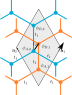
\includegraphics[width=0.3125\linewidth]{figures/bilayer.pdf}
\caption[]{Crystal structure and hoppings of AB-stacked bilayer graphene.}
\label{fig:bilayer}
\end{figure}
%
The main features of the model are its 4-atom unit cell spanned by vectors
$\mathbf{a}_1 = (1/2, \sqrt{3}/2)$ and $\mathbf{a}_2=( -1/2, \sqrt{3}/2)$,
and with wave functions $\phi_{A,1}, \phi_{B,1}, \phi_{A,2}, \phi_{B,2}$, where
$A$ and $B$ indices are the two sublattices, and $1,2$ are the layers.
The model has hoppings $t_1$ and $t_2$ within and between the layers,
respectively, as shown in Fig.~\ref{fig:bilayer}.
We also include a layer-dependent onsite potential $\pm m$.

\co{We use sympy.}
We define the Bloch Hamiltonian using the Sympy package for symbolic Python
\cite{Meurer_2017}.
%
\begin{minted}{ipython}
t_1, t_2, m = sympy.symbols("t_1 t_2 m", real=True)
alpha = sympy.symbols(r"\alpha")

H = Matrix([
    [m, t_1 * alpha, 0, 0],
    [t_1 * alpha.conjugate(), m, t_2, 0],
    [0, t_2, -m, t_1 * alpha],
    [0, 0, t_1 * alpha.conjugate(), -m]]
)
\end{minted}

$$
H =
\begin{pmatrix}
m & t_1 \alpha & 0 & 0\\
t_1 \alpha^{*} & m & t_2 & 0\\
0 & t_2 & -m & t_1 \alpha\\
0 & 0 & t_1 \alpha^{*} & -m
\end{pmatrix}
$$
%
where $\alpha(\mathbf{k}) = 1 + e^{i \mathbf{k} \cdot \mathbf{a}_1} + e^{\mathbf{k} \cdot
\mathbf{a}_2}$, with $k$ the wave vector.
We consider $\mathbf{K}=(4\pi/3, 0)$ the reference point point in $\mathbf{k}$-space:
$\mathbf{k} = (4\pi/3 + k_x, k_y)$ because $\alpha(\mathbf{K}) = 0$, making
$k_x$ and $k_y$ small perturbations.
Additionally, we consider $m \ll t_2$ a perturbative parameter.

\co{We define the perturbative series}
To call \mintinline{python}|block_diagonalize|, we need to define the subspaces
for the block diagonalization, so we compute the eigenvectors of the
unperturbed Hamiltonian at the $\mathbf{K}$ point, $H(\alpha(\mathbf{K}) = m =
0)$.
Then, we substitute $\alpha(\mathbf{k})$ into the Hamiltonian, and call the
block diagonalization routine using that $k_x$, $k_y$, and $m$ are perturbative
parameters via the \mintinline{Python}|symbols| argument.
%
\begin{minted}{python}
vecs = H.subs({alpha: 0, m: 0}).diagonalize(normalize=True)[0]

H_tilde, U, U_adjoint = block_diagonalize(
    H.subs({alpha: alpha_k}),
    symbols=(k_x, k_y, m),
    subspace_eigenvectors=[vecs[:, :2], vecs[:, 2:]]
)
\end{minted}
%
The order of the variables in the perturbative series will be that of
\mintinline{python}{symbols}.
For example, requesting the term $\propto k_x^{i} k_y^{j} m^{l}$ from the
effective model is done by calling \mintinline{python}|H_tilde[0, 0, i, j, l]|,
where the first two indices are the block indices (AA).
The series of the unitary transformation $U$ and $U^\dagger$ are also defined,
and we may use them to transform other operators.

We collect corrections up to third order in momentum to compute the standard
quadratic dispersion of bilayer graphene and trigonal warping.
We query these terms from \mintinline{Python}|H_tilde| and those proportional
to mass to obtain the effective Hamiltonian (shown as produced by the
code)\footnote{The full code is available at
\url{https://pymablock.readthedocs.io/en/latest/tutorial/bilayer_graphene.html}.}:
%
{\small
\begin{gather}
\tilde{H}_{\textrm{eff}} =
\begin{bmatrix}
m & \frac{3 t_1^2}{4 t_2} ( - k_x^2 - 2ik_x k_y + k_y^2) \\
\frac{3 t_1^2}{4 t_2} ( - k_x^2 + 2ik_x k_y + k_y^2) & -m
\end{bmatrix} + \nonumber \\
\begin{bmatrix}
\frac{3 m t_1^2}{2 t_2^2} ( - k_x^2 - k_y^2) & \frac{\sqrt{3} t_1^2}{8 t_2} (k_x^3 - 5ik_x^2 k_y + 9 k_x k_y^2 + 3ik_y^3) \\
\frac{\sqrt{3} t_1^2}{8 t_2} (k_x^3 + 5ik_x^2 k_y + 9 k_x k_y^2 - 3ik_y^3) & \frac{3 m t_1^2}{2 t_2^2} (k_x^2 + k_y^2)
\end{bmatrix} \nonumber
\end{gather}
}
%
The first term is the standard quadratic dispersion of gapped bilayer
graphene.
The second term contains trigonal warping and the coupling between the gap and
momentum.
All the terms take less than two seconds in a personal computer to compute.

\subsection{Induced gap in a double quantum dot}

\co{Large systems pose an additional challenge due to the scaling of linear
algebra routines for large matrices.}
Large systems pose an additional challenge due to the cubic scaling of linear
algebra routines with matrix size.
To overcome this, Pymablock is equipped with an implicit method, which utilizes
the sparsity of the input and avoids the construction of the full transformed
Hamiltonian.
We illustrate the efficiency of this method by applying it to a system of two
quantum dots coupled to a superconductor between them, shown in
Fig.~\ref{fig:QD_spectrum}, and described by the Bogoliubov-de Gennes Hamiltonian:
%
\begin{equation}
    H_{BdG} =
    \begin{cases}
        (\mathbf{k}^2/2m - \mu_{sc}) \sigma_z + \Delta \sigma_x \quad & \text{for } L/3 \leq x \leq 2L/3, \\
        (\mathbf{k}^2/2m - \mu_n) \sigma_z \quad & \text{otherwise},
    \end{cases}
\end{equation}
where the Pauli matrices $\sigma_z$ and $\sigma_x$ act in the electron-hole
space, $\mathbf{k}$ is the 2D wave vector, $m$ is the effective mass, and
$\Delta$ the superconducting gap.

\co{We use Kwant to build the Hamiltonian of the system.}
We use the Kwant package~\cite{Groth_2014} to build the Hamiltonian of the
system~\footnote{The full code is available at
\url{https://pymablock.readthedocs.io/en/latest/tutorial/induced_gap.html}.},
which we define over a square lattice of $L \times W = 200 \times 40$ sites.
On top of this, we consider two perturbations: the barrier strength between the
quantum dots and the superconductor, $t_b$, and an asymmetry of
the dots potentials, $\delta \mu$.

The system is large: it is a sparse array of size $63042 \times 63042$, with
$333680$ non-zero elements, so even storing all the eigenvectors would take
$60$ GB of memory.
The perturbations are also sparse, with $632$, and $126084$ non-zero elements
for the barrier strength and the potential asymmetry, respectively.
The sparsity structure of the Hamiltonian and the perturbations is shown in the
left panel of Fig.~\ref{fig:QD_spectrum}, where we use a smaller system of $L
\times W = 8 \times 2$ for visualization.
Therefore, we use sparse diagonalization and compute only four eigenvectors of
the unperturbed Hamiltonian closest to zero energy, which are the Andreev
states of the quantum dots.
%
\inputminted[firstline=62, lastline=63]{ipython}{code_figures/lattice_system.py}
%
We now call the block diagonalization routine and provide the computed
eigenvectors.
%
\inputminted[firstline=65, lastline=65]{ipython}{code_figures/lattice_system.py}
%
Because we only provide the low energy subspace, Pymablock uses the implicit
method.
Calling \mintinline{python}|block_diagonalize| is now the most time consuming
step because it requires pre-computing several decompositions of the full
Hamiltonian.
It is, however, manageable and it only produces a constant overhead of less
than three seconds.

To compute the spectrum, we collect the lowest three orders in each parameter
in an appropriately sized tensor.
%
\inputminted[firstline=71, lastline=71]{ipython}{code_figures/lattice_system.py}
%
This takes two more seconds to run, and we can now compute the low energy
spectrum after rescaling the perturbative corrections by the magnitude of each
perturbation.
%
\inputminted[firstline=74, lastline=79]{ipython}{code_figures/lattice_system.py}
%
Finally, we plot the spectrum in Fig.~\ref{fig:QD_spectrum}.
%
\begin{figure}[h!]
\centering
\includegraphics[width=\linewidth]{figures/lattice_system.pdf}
\caption{
    Low energy spectrum of two quantum dots coupled to a superconductor for
    three values of the barrier strength $t_b \in (0, 0.5, 0.75)$.
}
\label{fig:QD_spectrum}
\end{figure}
%
As expected, the crossing at $E=0$ due to the dot asymmetry is lifted when the
dots are coupled to the superconductor.
In addition, we observe how the proximity gap of the dots increases with the
coupling strength.

In this example the total runtime of Pymablock would only allow us to compute
the spectrum at around $3$ points in the parameter space.
This demonstrates the speed of the implicit method and the efficiency of
Pymablock's algorithm.

\subsection{CQED}

\section{Pymablock's algorithm}

\subsection{Problem statement}

Pymablock finds a series of the unitary transformation $\mathcal{U}$ (we use
calligraphic letters to denote series) that block-diagonalizes the Hamiltonian
%
\begin{align}
\label{hamiltonian}
\mathcal{H} = H_0 + \mathcal{H}',\quad H_0 = \begin{pmatrix}
H_0^{AA} & 0\\
0 & H_0^{BB}
\end{pmatrix},
\end{align}
%
with $\mathcal{H}'$ containing an arbitrary number and orders of perturbations.
The series here may be multivariate, and they represent sums of the form
%
\begin{align}
\mathcal{A} = \sum_{n_1=0}^\infty \sum_{n_2=0}^\infty \cdots \sum_{n_k=0}^\infty \lambda_1^{n_1} \lambda_2^{n_2} \cdots \lambda_k^{n_k} A_{n_1, n_2, \ldots, n_k},
\end{align}
%
where $\lambda_i$ are the perturbation parameters and $A_{n_1, n_2, \ldots,
n_k}$ are linear operators.
%
The problem statement, therefore, is finding $\mathcal{U}$ and
$\tilde{\mathcal{H}}$ such that
%
\begin{align}
\label{eq:problem_definition}
\tilde{\mathcal{H}} = \mathcal{U}^\dagger \mathcal{H} \mathcal{U},\quad \tilde{\mathcal{H}}^{AB} = 0,\quad \mathcal{U}^\dagger \mathcal{U} = 1,
\end{align}
%
which is schematically shown in Fig.~\ref{fig:block_diagonalization}.
Series multiply according to the Cauchy product:
%
$$
\mathcal{C} = \mathcal{A}\mathcal{B} \Leftrightarrow C_\mathbf{n} = \sum_{\mathbf{m} + \mathbf{p} = \mathbf{n}} A_\mathbf{m} B_\mathbf{p}.
$$
%
The Cauchy product is the most expensive operation in perturbation theory,
because it involves a large number of multiplications between potentially large
matrices.
For example, evaluating $\mathbf{n}$-th order of $\mathcal{C}$ requires
$\sim\prod_i n_i \equiv N$ multiplications of the series elements.
A direct computation of all the possible index combinations in a product
between three series $\mathcal{A}\mathcal{B}\mathcal{C}$ would have a higher
cost $\sim N^2$, however if we use associativity of the product and compute
this as $(\mathcal{A}\mathcal{B})\mathcal{C}$, then the scaling of the cost
stays $\sim N$.
%
\begin{figure}[h!]
\centering
\includegraphics[width=\textwidth]{figures/diagrams_H.pdf}
\caption{
  Perturbative block-diagonalization of a gapped Hamiltonian with a first order
  perturbation.
  The effective Hamiltonian is the $2\times 2$ block in the top left corner in
  the last panel.
}
\label{fig:block_diagonalization}
\end{figure}

There are many ways to solve the problem~\eqref{eq:problem_definition} that
give identical expressions for $\mathcal{U}$ and $\tilde{\mathcal{H}}$.
We are searching for a procedure that satisfies two additional constraints:
%
\begin{itemize}
    \item It has the same complexity scaling as a Cauchy product.
    \item It does not require multiplications by $H_0$.
\end{itemize}
%
The second requirement is because in perturbation theory, $n$-th order  corrections to
$\tilde{\mathcal{H}}$ carry $n$ energy denominators $1/(E_i - E_j)$, where
$E_i$ and $E_j$ are the eigenvalues of $H_0$ belonging to different subspaces.
Therefore, any additional multiplications by $H_0$ must cancel with
additional energy denominators.
Multiplying by $H_0$ is therefore unnecessary work, and it gives longer
intermediate expressions.
The goal of our algorithm is thus to be efficient and to produce compact
results that do not require further simplifications.
\subsection{Existing solutions}
\co{Pymablock's algorithm does not use the Schrieffer--Wolff transformation,
because the former is inefficient.}
A common approach to construct effective Hamiltonians is to use the
Schrieffer--Wolff transformation~\cite{Schrieffer_1966}:
%
\begin{align}
\tilde{\mathcal{H}} = e^\mathcal{S} &\mathcal{H} e^{-\mathcal{S}}, \\
e^{\mathcal{S}} = 1 + \mathcal{S} + \frac{1}{2!} \mathcal{S} \mathcal{S}
+ &\frac{1}{3!} \mathcal{S} \mathcal{S} \mathcal{S} + \cdots,
\end{align}
%
where $\mathcal{S} = \sum_n S_n$ is an antihermitian polynomial series in the
perturbative parameter, making $e^\mathcal{S}$ a unitary transformation.
Requiring that $\tilde{\mathcal{H}}^{AB} = 0$ gives a recursive equation for
$S_n$, whose terms are nested commutators between the series of $\mathcal{S}$
and $\mathcal{H}$.
Similarly, the transformed Hamiltonian is given by a series of nested
commutators
%
\begin{equation}
\label{eq:SW_H}
\tilde{\mathcal{H}} = \sum_{j=0}^\infty \frac{1}{j!} \Big [\mathcal{H}, \sum_{n=0}^{\infty} S_n \Big ]^{(j)}.
\end{equation}
%
Regardless of the specific implementation, this expression does not meet either
of our two requirements:
\begin{itemize}
  \item The direct computation of the series elements requires a $\sim \exp N$
  multiplications, and even an optimized one has a $\sim N^2$ scaling.
  \item Evaluating Eq.~\eqref{eq:SW_H} contains multiplications by $H_0$.
\end{itemize}

\co{There are algorithms that use different parametrizations for U a
difference that is crucial for efficiency, even though the results are
equivalent.}
Alternative parametrizations of the unitary transformation $\mathcal{U}$
require solving unitarity and block diagonalization conditions too, but
give rise to a different recursive procedure for the series elements.
For example, using hyperbolic functions
%
\begin{gather}
\mathcal{U} = \cosh{\mathcal{G}} + \sinh{\mathcal{G}}, \quad
\mathcal{G} = \sum_{i=0}^{\infty} G_i,
\end{gather}
%
leads to different recursive expressions for $G_i$ \cite{Shavitt_1980},
but does not change the algorithm's complexity.
On the other hand, using a polynomial series directly
%
\begin{align}
\mathcal{U} &= \sum_{i=0}^{\infty} U_i,
\end{align}
%
gives rise to another recursive equation for $U_i$
\cite{Van_Vleck_1929, Lowdin_1962, Klein_1974, Suzuki_1983}.
Still, this choice results in an expression for $\tilde{\mathcal{H}}$ whose
terms include products by $H_0$, and therefore requires additional
simplifications.

\co{The existing algorithms with linear scaling are not suitable for the
construction of an effective Hamiltonian.}
Despite the conceptual equivalence of the algorithms and the agreement of their
results, there is a crucial difference in their computational efficiency: a
Schrieffer--Wolff transformation has an exponential scaling with the
perturbative order, but it can be reduced.
C. Bloch's perturbation theory \cite{Bloch_1958}, for example,
aims to find a similarity transform that brings the Hamiltonian to a
block-triangular form, losing its Hermiticity and orhogonality properties.
The iterative procedure to find the similarity transform requires computing
fewer expressions for the series elements than the Schrieffer-Wolff
transformation \cite{Bravyi_2011}, and the effective Hamiltonian is more
compact.
However, the algorithm is only useful to obtain the spectrum of the low energy
subspace, not its wavefunctions.
Reference \cite{Li_2022}, for example, introduces an
algorithm with linear scaling for diagonalization of a single state by
reformulating the recursive steps of the Schrieffer--Wolff transformation.
Block diagonalization of a Hamiltonian, however, recovers the exponential
scaling.
Another approach with linear scaling is that of density matrix perturbation
theory \cite{McWeeny_1962,McWeeny_1968,Truflandier_2020}, in which the
density matrix of a single-particle system is also a power series with
respect to a perturbative parameter:
%
\begin{align}
  \mathcal{D} = \sum_{i=0}^{\infty} D_i.
\end{align}
%
The elements of the series are found by solving two recursive conditions,
$\mathcal{D}^2 = \mathcal{D}$ and $[\mathcal{H}, \mathcal{D}]=0$.
This approach, however, does not provide an effective Hamiltonian, and even
though it has a linear scaling, it deals with the entire Hilbert space, not
only the low energy subspace.
We thus identify the need for an algorithm that combines linear scaling with
the ability to construct an effective Hamiltonian.

\subsection{Our solution}

To find $\mathcal{U}$, let us separate it into an identity and $\mathcal{U}' =
\mathcal{W} + \mathcal{V}$:
%
\begin{align}
\label{eq:U}
\mathcal{U} = 1 + \mathcal{U}' = 1 + \mathcal{W} + \mathcal{V},\quad \mathcal{W}^\dagger = \mathcal{W},\quad \mathcal{V}^\dagger = -\mathcal{V}.
\end{align}
%
First, we use the unitarity condition
$\mathcal{U}^\dagger \mathcal{U} = 1$ by substituting $\mathcal{U}'$ into it
and obtain
%
\begin{align}
\label{eq:W}
\mathcal{W} &= \frac{1}{2}(\mathcal{U}'^\dagger + \mathcal{U}') \nonumber \\
  &= \frac{1}{2} \Big[(1 + \mathcal{U}'^\dagger)(1+\mathcal{U}') - 1 - \mathcal{U}'^\dagger \mathcal{U}' \Big] \nonumber \\
  &= -\frac{1}{2} \mathcal{U}'^\dagger \mathcal{U}'.
\end{align}
%
Because $\mathcal{U}'$ has no $0$-th order term, $(\mathcal{U}'^\dagger
\mathcal{U}')_\mathbf{n}$ does not depend on the $\mathbf{n}$-th order of
$\mathcal{U}'$ nor $\mathcal{W}$.
More generally, a Cauchy product $\mathcal{A}\mathcal{B}$ where $\mathcal{A}$
and $\mathcal{B}$ have no $0$-th order terms depends on $\mathcal{A}_1, \ldots,
\mathcal{A}_{n-1}$ and $\mathcal{B}_1, \ldots, \mathcal{B}_{n-1}$.
This allows us to use Cauchy products to define recurrence relations, which
we apply throughout the algorithm.
Therefore, we compute $\mathcal{W}$ as a Cauchy product of $\mathcal{U}'$ with
itself \footnotemark[1].

\footnotetext[1]{
Using the definition of $\mathcal{W}$ as the Hermitian part of $\mathcal{U}'$,
and the unitarity condition:
%
$$
2\mathcal{W}
= \mathcal{U}' + \mathcal{U}'^\dagger
= -\mathcal{U}'^\dagger \mathcal{U}'
= -\mathcal{W}^2 + \mathcal{V}^2.
$$
%
we see that we could alternatively define $\mathcal{W}$ as a Taylor series in
$\mathcal{V}$:
%
$$
\mathcal{W} = \sqrt{1 + \mathcal{V}^2} - 1 \equiv f(\mathcal{V}) \equiv \sum_n a_n \mathcal{V}^{2n},
$$
%
however the scaling of such a Cauchy product becomes slower if we need to
compute a Taylor expansion of a series.
A direct computation of all possible products of terms would require $\sim \exp
N$ multiplications.
We improve on this by defining a new series as $\mathcal{A}^{n+1} =
\mathcal{A}\mathcal{A}^{n}$ and reusing the previously computed results, which
brings these costs down to $\sim N^2$.
Using the Taylor expansion approach is therefore both more complicated and more
computationally expensive than the recurrent definition in Eq.~\eqref{eq:W}.
}

To compute $\mathcal{U}'$ we also need to find $\mathcal{V}$, which is defined
by the requirement $\tilde{\mathcal{H}}^{AB} = 0$.
Additionally, we constrain $\mathcal{V}$ to be block off-diagonal:
$\mathcal{V}^{AA} = \mathcal{V}^{BB} = 0$,
so that the resulting unitary transformation is equivalent to the
Schrieffer--Wolff transformation.
In turn, this means that $\mathcal{W}$ is block-diagonal and that the norm
of $\mathcal{U}'$ is minimal.

\co{We find V and the transformed Hamiltonian.}
To find $\mathcal{V}$, we need to first look at the transformed Hamiltonian:
%
\begin{align}
\tilde{\mathcal{H}} = \mathcal{U}^\dagger \mathcal{H} \mathcal{U} = H_0 +
\mathcal{U}'^\dagger H_0 + H_0 \mathcal{U}' + \mathcal{U}'^\dagger H_0
\mathcal{U}' + \mathcal{U}^\dagger\mathcal{H'}\mathcal{U},
\end{align}
%
where we used $\mathcal{U}=1+\mathcal{U}'$ and $\mathcal{H} = H_0 +
\mathcal{H'}$.
Because we want to avoid unnecessary products by $H_0$, we need to get rid of
the terms that contain it by replacing them with an alternative expression.
Our strategy is to define an auxiliary operator $\mathcal{X}$ that we can
compute without ever multiplying by $H_0$.
Like $\mathcal{U}'$, $\mathcal{X}$ needs to be defined via a recurrence
relation, which we will find later.
Because the expression above has $H_0$ multiplied by $\mathcal{U}'$ by the left
and by the right, we get rid of these terms by making sure that $H_0$
multiplies terms from one side only.
To achieve this, we choose $\mathcal{X}=\mathcal{Y}+\mathcal{Z}$ to be the commutator between
$\mathcal{U}'$ and $H_0$:
%
\begin{align}
\label{eq:XYZ}
\mathcal{X} \equiv [\mathcal{U}', H_0] = \mathcal{Y} + \mathcal{Z}, \quad
\mathcal{Y} \equiv [\mathcal{V}, H_0] = \mathcal{Y}^\dagger,\quad
\mathcal{Z} \equiv [\mathcal{W}, H_0] = -\mathcal{Z}^\dagger,
\end{align}
%
where $\mathcal{Y}$ is therefore block off-diagonal and $\mathcal{Z}$, block
diagonal.
We use $H_0 \mathcal{U}' = \mathcal{U}' H_0 -\mathcal{X}$ to move $H_0$ through
to the right and find
%
\begin{align}
\label{eq:H_tilde}
  \tilde{\mathcal{H}}
  &= H_0 + \mathcal{U}'^\dagger H_0 + (H_0 \mathcal{U}') + \mathcal{U}'^\dagger H_0
  \mathcal{U}' + \mathcal{U}^\dagger(\mathcal{H'}\mathcal{U}) \nonumber
  \\
  &= H_0 + \mathcal{U}'^\dagger H_0 + \mathcal{U}'H_0 - \mathcal{X} + \mathcal{U}'^\dagger (\mathcal{U}' H_0 - \mathcal{X}) + \mathcal{U}^\dagger\mathcal{H'}\mathcal{U} \nonumber \\
  &= H_0 + (\mathcal{U}'^\dagger + \mathcal{U}' + \mathcal{U}'^\dagger \mathcal{U}')H_0 - \mathcal{X} - \mathcal{U}'^\dagger \mathcal{X} + \mathcal{U}^\dagger\mathcal{H'}\mathcal{U} \nonumber \\
  &= H_0 - \mathcal{X} - \mathcal{U}'^\dagger \mathcal{X} + \mathcal{U}^\dagger\mathcal{H'}\mathcal{U},
\end{align}
%
where the terms multiplied by $H_0$ cancel by unitarity.

\missingfigure{Show block structure of series.}

The transformed Hamiltonian does not contain products by $H_0$ anymore, but it
does depend on $\mathcal{X}$, an auxiliary operator whose recurrent definition
we do not know yet.
To find it, we first focus on its anti-Hermitian part, $\mathcal{Z}$.
Since recurrence relations are expressions whose right hand side contains
Cauchy products between series, we need to find a way to make a product appear.
We do so by using the unitarity condition $\mathcal{U}'^\dagger + \mathcal{U}' =
-\mathcal{U}'^\dagger \mathcal{U}'$ to rewrite $\mathcal{Z}$:
%
\begin{align}
\label{eq:Z}
\mathcal{Z}
&= \frac{1}{2} (\mathcal{X} - \mathcal{X}^{\dagger}) \nonumber \\
&= \frac{1}{2}\Big[ (\mathcal{U}' + \mathcal{U}'^{\dagger}) H_0 - H_0 (\mathcal{U}' + \mathcal{U}'^{\dagger}) \Big] \nonumber \\
&= \frac{1}{2} \Big[ - \mathcal{U}'^{\dagger} (\mathcal{U}'H_0 - H_0 \mathcal{U}') + (\mathcal{U}'H_0 - H_0 \mathcal{U}')^{\dagger} \mathcal{U}' \Big] \nonumber \\
&= \frac{1}{2} (-\mathcal{U}'^{\dagger} \mathcal{X} + \mathcal{X}^{\dagger} \mathcal{U}').
\end{align}
%
Similar to computing $W_{\mathbf{n}}$, computing $Z_{\mathbf{n}}$ requires lower orders of
$\mathcal{X}$ and $\mathcal{U}'$, all blocks included.
This defines a recursive relation for $\mathcal{Z}$.
Then, we compute the Hermitian part of $\mathcal{X}$ by requiring that
$\tilde{\mathcal{H}}^{AB} = 0$ and find
%
\begin{align}
\label{eq:Y}
\mathcal{X}^{AB} = (\mathcal{U}^\dagger \mathcal{H}' \mathcal{U} -
\mathcal{U}'^\dagger \mathcal{X})^{AB}.
\end{align}
%
Once again, despite $\mathcal{X}$ enters the right hand side, because all the
terms lack \nth{0} order, this defines a recursive relation for $\mathcal{X}^{AB}$,
and therefore $\mathcal{Y}$.

The final part is standard: the definition of $\mathcal{Y}$ in
Eq.~\eqref{eq:XYZ} fixes $\mathcal{V}$ as a solution of:
%
\begin{align}
\label{eq:sylvester}
\mathcal{V}^{AB}H_0^{BB} - H_0^{AA} \mathcal{V}^{AB} = \mathcal{Y}^{AB},
\end{align}
%
a Sylvester's equation, which we only need to solve once for every new order.
In the eigenbasis of $H_0$, the solution of Sylvester's equation is
$V^{AB}_{\mathbf{n}, ij} = Y^{AB}_{\mathbf{n}, ij}/(E_i - E_j)$, where $E_i$ are the eigenvalues of
$H_0$.
However, even if the eigenbasis of $H_0$ is not available, there are efficient
algorithms to solve Sylvester's equation, see below.

\subsection{Algorithm}

We now have the complete algorithm:
%
\begin{enumerate}
    \item Define series $\mathcal{U}'$ and $\mathcal{X}$ and make use of their block structure and Hermiticity.
    \item To define the diagonal blocks of $\mathcal{U}'$, use $\mathcal{W} = -\mathcal{U}'^\dagger\mathcal{U}'/2$.
    \item To find the off-diagonal blocks of $\mathcal{U}'$, solve Sylvester's equation $\mathcal{V}^{AB}H_0^{BB} - H_0^{AA}\mathcal{V}^{AB} = \mathcal{Y}^{AB}$.
      This requires $\mathcal{X}$.
    \item To find the diagonal blocks of $\mathcal{X}$, define $\mathcal{Z} = (-\mathcal{U}'^\dagger\mathcal{X} + \mathcal{X}^\dagger\mathcal{U}')/2$.
    \item For the off-diagonal blocks of $\mathcal{X}$, use $\mathcal{Y}^{AB} =
    (-\mathcal{U}'^\dagger\mathcal{X} +
     \mathcal{U}^\dagger\mathcal{H}'\mathcal{U})^{AB}$.
    \item  Compute the effective Hamiltonian as $\tilde{\mathcal{H}}_{\textrm{diag}} = H_0 - \mathcal{X} - \mathcal{U}'^\dagger \mathcal{X} + \mathcal{U}^\dagger\mathcal{H'}\mathcal{U}$.
\end{enumerate}

\subsection{Equivalence with Schrieffer--Wolff transformation}
\co{Our algorithm is equivalent to a Schrieffer--Wolff transformation}
Both the Pymablock algorithm and the more commonly used Schrieffer-Wolff
transformation find a unitary transformation $\mathcal{U}$ such that
$\tilde{\mathcal{H}}^{AB}=0$.
They are therefore equivalent up to a gauge choice in each subspace, $A$ and
$B$.

We establish the equivalence between the two by demonstrating that this gauge
choice is the same for both algorithms.
The Schrieffer--Wolff transformation uses $\mathcal{U} = \exp \mathcal{S}$,
where $\mathcal{S} = -\mathcal{S}^\dagger$ and $\mathcal{S}^{AA} =
\mathcal{S}^{BB} = 0$.
The series $\exp\mathcal{S}$ contains all possible products of $S_n$ of all
lengths with fractional prefactors.
For every term $S_{k_1}S_{k_2}\cdots S_{k_n}$, there is a corresponding term
$S_{k_n}S_{k_{n-1}}\cdots S_{k_1}$ with the same prefactor.
If the number of $S_{k_n}$ is even, then both terms are block-diagonal since
each $S_n$ is block off-diagonal.
Because $S_n$ are anti-Hermitian, the two terms are Hermitian conjugates of each
other, and therefore their sum is Hermitian.
On the other hand, if the number of $S_{k_n}$ is odd, then the two terms are
block off-diagonal and their sum is anti-Hermitian by the same reasoning.
Therefore, just like in our algorithm, the diagonal blocks of $\exp S$ are
Hermitian, while off-diagonal blocks are anti-Hermitian.
Schrieffer--Wolff transformation produces a unique answer and satisfies the same
diagonalization requirements as our algorithm, which means that the two produce
the same effective Hamiltonian.

\subsection{Extra optimization: common subexpression elimination}
%
We further optimize the algorithm by reusing products that are needed in several
places.
%
Firstly, we rewrite the expressions for $\mathcal{Z}$ and $\tilde{\mathcal{H}}$
by utilizing the Hermitian conjugate of $\mathcal{U}'^\dagger \mathcal{X}$ without recomputing it:
%
\begin{gather*}
\mathcal{Z} = \frac{1}{2}[(-\mathcal{U}'^\dagger \mathcal{X})- \textrm{h.c.}],\\
\tilde{\mathcal{H}} = H_0 + \mathcal{U}^\dagger \mathcal{H}' \mathcal{U} - (\mathcal{U}'^\dagger \mathcal{X} + \textrm{h.c.}),
\end{gather*}
%
where $\textrm{h.c.}$ is the Hermitian conjugate, and $\mathcal{X}$ drops out from the diagonal blocks of $\tilde{\mathcal{H}}$ because diagonal of $\mathcal{X}$ is anti-Hermitian.
%
To compute $\mathcal{U}^\dagger \mathcal{H}' \mathcal{U}$ faster, we express it
using $\mathcal{F} \equiv \mathcal{H}'\mathcal{U}'$:
%
$$
\mathcal{U}^\dagger \mathcal{H}' \mathcal{U} = \mathcal{H}' + \mathcal{F} + \mathcal{F}^\dagger + \mathcal{U}'^\dagger \mathcal{F}.
$$
%
To further optimize the computations, we observe that some products appear both in $\mathcal{U}'^\dagger \mathcal{X}$ and $\mathcal{U}^\dagger \mathcal{H}' \mathcal{U}$.
%
To reuse these products, we separate the perturbation into diagonal and off-diagonal parts $\mathcal{H}' = \mathcal{H}'_\textrm{diag} + \mathcal{H}'_\textrm{offdiag}$.
%
We then introduce variables
%
\begin{align}
\mathcal{A} = \mathcal{H}'_\textrm{diag} \mathcal{U}', \quad
\mathcal{B} = \mathcal{H}'_\textrm{offdiag} \mathcal{U}', \quad
\mathcal{C} = \mathcal{X} - \mathcal{H}'_\textrm{offdiag}
\end{align}
%
This gives an updated expression for $\mathcal{Z}$:
%
\begin{align}
\label{eq:Z_optimized}
\mathcal{Z} = \frac{1}{2}(\mathcal{B}^\dagger - \mathcal{U}^\dagger\mathcal{C}) - \textrm{h.c.},
\end{align}
%
and more importantly for $\tilde{\mathcal{H}}$:
%
\begin{align}
\label{eq:H_tilde_optimized}
\tilde{\mathcal{H}} = H_0 + \mathcal{A} + \mathcal{A}^\dagger + (\mathcal{B} + \mathcal{B}^\dagger)/2 + \mathcal{U}'^\dagger (\mathcal{A} + \mathcal{B}) - (\mathcal{U}^\dagger \mathcal{C} + \textrm{h.c.})/2.
\end{align}

\section{Implementation}

\co{To implement the algorithms, we need a data structure that represents a
multidimensional series of block matrices.}
To implement the algorithm, we need a data structure that represents a
multidimensional series of operators, where dimensions label independent
perturbations.
Additionally, the data structure needs to label blocks, so that the algorithm
supports several forms of input, e.g. dense arrays, sparse matrices, symbolic
expressions, an implicit subspace, or a custom Python object that supports
products and sums.
Manipulating blocks also allows to compute the effective Hamiltonian without
explicitly constructing the full Hamiltonian, which is useful for Hamiltonians
with a large $BB$ subspace that is costly to store and compute.
To run the recursion, the series needs to be queryable by order and block.
This is also useful in cases where the user may want terms that combine
different perturbations, or when the user wants to compute more terms than
originally requested.
Lastly, the data structure needs to support a block-wise multivariate Cauchy
product, which is the main operation in the recursion and is used to compute
the transformed Hamiltonian.

\co{We address this by defining a BlockSeries class.}
To address these requirements, we define a \mintinline{python}|BlockSeries|
Python class and use it to represent the series of $\mathcal{U}$,
$\mathcal{H}$, and $\tilde{\mathcal{H}}$.
The objects of this class are equipped with a function to compute their elements
and a dictionary to cache the results.
For example, the \mintinline{python}|BlockSeries| for $\tilde{\mathcal{H}}$ has
a function that computes the block-wise multivariate Cauchy product in
Eq.~\eqref{eq:H_tilde_optimized}, \mintinline{python}|compute_H_tilde|.
%
\begin{minted}{python}
    H_tilde = BlockSeries(
        shape=(2, 2), # 2 blocks
        n_infinite=1, # number of perturbative parameters
        eval=compute_H_tilde,
        name="H_tilde",
        dimension_names=("lambda",),
    )
\end{minted}
%
To get the elements of the series, we implement Numpy array indexing,
which allows us to request several elements at once by using tuples and slices.
\mintinline{python}|H_tilde[0, 0, 2]| returns the $AA$ block of
$\tilde{\mathcal{H}}$ proportional to $\lambda^2$, and
\mintinline{python}|H_tilde[0, 0, :3]| returns the $AA$ block of orders
$\lambda^0$ , $\lambda^1$, and $\lambda^2$ in a Numpy masked array.
In the latter, the masked array only contains non-zero elements, a feature that
we use each time we compute the Cauchy products between series, avoiding
unnecessary matrix products.

\co{Using the BlockSeries interface allows us to implement a range of
optimizations that go beyond directly implementing the polynomial
parametrization}
Not only does the \mintinline{python}|BlockSeries| interface allow us to
implement the polynomial parametrization of the unitary transformation, but
also several other optimizations.
For example, we exploit Hermiticity when computing the Cauchy product of
$U'^{\dagger}U'$ in Eq.~\eqref{eq:W}, for which we only need to compute half of
the matrix products that form its diagonal blocks, and then complex conjugate
the result to obtain the rest.
Similarly, for Hermitian and anti-Hermitian series, like the off-diagonal
blocks of $\mathcal{X} - \mathcal{H}'_\textrm{offdiag}$ and off-diagonal blocks
of $\mathcal{U}'$, we only compute the $AB$ blocks, and use the conjugate
transpose to obtain the $BA$ blocks.
This is only one example of how the \mintinline{python}|BlockSeries| interface
allows us to implement a symmetrized algorithm, and we leave other symmetries
for future work.
Such an extension would be useful for systems where $\mathcal{U}$ or
$\tilde{\mathcal{H}}$ vanish due to symmetries, so that the zero blocks can be
skipped beforehand.

\co{A key optimization that BlockSeries enable is the implicit treatpapment
of the BB subspace.}
Solving Sylvester's equation and computing the matrix products are the most
expensive steps of the algorithms for large Hamiltonians.
Pymablock can efficiently construct an effective Hamiltonian of a small
subspace even when the full Hamiltonian is a sparse matrix that is too costly to
diagonalize.
It does so by avoiding explicit computation of operators in $B$ subspace, and
by utilizing the sparsity of the Hamiltonian to compute the Green's function,
which is the solution of Sylvester's equation.
To do so, Pymablock uses either the MUMPS sparse solver via the python-mumps
wrapper or the KPM method, an approach originally introduced in
references~\cite{Weisse_2006, Irfan_2019}.


\co{To deal with an implicit B subspace, we use MUMPS and LinearOperators.}
Because \mintinline{python}|BlockSeries| can represent any input type, we use
it to directly implement the implicit algorithm for large sparse Hamiltonians.
To do this, we use the matrix $\Psi_A$ of the eigenvectors of the $A$ subspace
to rewrite the Hamiltonian as
%
\begin{align}
\mathcal{H} \to \begin{pmatrix}
\Psi_A^\dagger \mathcal{H} \Psi_A & \Psi_A^\dagger \mathcal{H} P_B \\
P_B \mathcal{H} \Psi_A & P_B \mathcal{H} P_B
\end{pmatrix},
\end{align}
%
where $P_B = 1 - \Psi_A \Psi_A^\dagger$ is the projector onto the $B$ subspace.
This Hamiltonian is larger in size than the original one because the $B$ block
has additional null vectors corresponding to the $A$ subspace.
This, however, allows to preserve the sparsity structure of the Hamiltonian by
applying $P_B$ and $\mathcal{H}$ separately.
Additionally, applying $P_B$ is efficient because $\Psi_A$ is a low rank matrix.
We then perform perturbation theory of the rewritten $\mathcal{H}$.
To solve the Sylvester's equation for the modified Hamiltonian, we write it for
every row of $V_n^{AB}$ separately:
%
\begin{align}
V_{n, ij}^{AB} (E_i - H_0) = Y_{n, j}
\end{align}
%
This equation is well-defined despite $E_i - H_0$ is not invertible because
$Y_{n}$ has no components in the $A$ subspace.
Here we also wrap the projector $P_B$ by a \mintinline{python}{LinearOperator}
object from \mintinline{python}{Scipy}.
This allows us to compute matrix-vector products between $P_B$ and a vector,
without explicitly constructing $P_B$ or any other product between elements of
the $B$ subspace, keeping the memory usage low.
For the same purpose, we use the MUMPS sparse solver \cite{Amestoy_2001},
\cite{Amestoy_2006}, or the KPM method \cite{Weisse_2006}, to compute the
Green's function of the $B$ subspace.
As a consequence, the implicit algorithm can be used on matrices with millions
of degrees of freedom as long as they are sparse.

\co{Finally, we implement an overall function that interprets the user inputs and
returns a BlockSeries for the transformed Hamiltonian.}
On the other hand, the standard algorithm explicitly manipulates both subspaces,
but can work with dense matrices too.
We use the eigenvectors of the $A$ and $B$ subspaces to project the input
Hamiltonian and represent it with a \mintinline{python}|BlockSeries|, a
procedure that works for numerical and symbolic matrices.
Because we aim for an easy-to-use interface, we implement a function that
interprets the user inputs and decides which algorithm to use: the implicit
method if only the $A$ subspace is provided, and the standard algorithm
otherwise.
This is \mintinline{python}|block_diagonalize|, the only function that the user
needs to call.
If $H_0$ is diagonal and a custom function to solve Sylvester's equation is not
provided to \mintinline{python}|block_diagonalize|, Pymablock uses a default
function to compute the energy denominators.

\section{Benchmark}
\label{sec:benchmark}

\co{Pymablock is more efficient than a direct implementation of a Schrieffer--Wolff transformation.}
To the best of our knowledge, there are no other packages implementing arbitrary order quasi-degenerate perturbation theory.
Literature references provide explicit expressions for the effective Hamiltonian up to fourth order, together with the procedure for obtaining higher order expressions~\cite{Winkler_2003}.
Because the full reference expressions are lengthy, we do not provide them, but for example at $4$-th order the effective Hamiltonian is a sum of several expressions of the form
\begin{equation}
\label{eq:SW_term}
\sum_{m^{''} m^{'''} l}
\frac{H'_{mm^{''}}H'_{m^{''}m^{'''}}H'_{m^{'''}l}H'_{lm^{'}}}{(E_{m^{''}}-E_{l})(E_{m^{'''}}-E_{l})(E_{m}-E_{l})},
\end{equation}
where the $m$-indices label states from the $A$-subspace and $l$-indices label the states from the $B$-subspace.
More generally, at $n$-th order each term is a product of $n$ matrix elements of the Hamiltonian and $n-1$ energy denominators.
Directly carrying out the summation over all the states requires $\mathcal{O}(N_A^2 N_B^{n-1})$ operations, where $N_A$ and $N_B$ are the number of states in the two subspaces.
In other words, the direct computation scales worse than a matrix product with the problem size.
Formulating Eq.~\eqref{eq:SW_term} as $n-1$ matrix products combined with $n-1$ solutions
of Sylvester's equation, brings this complexity down to $\mathcal{O}((n-1) \times N_A N_B^2)$.
This optimization, together with the hermiticity of the sum, allows us to evaluate the reference expressions for the effective Hamiltonian for $2$-nd, $3$-rd, and $4$-th order using $1$, $4$, and $27$ matrix products, respectively.
Pymablock's algorithm utilizes $1$, $3$, and $14$, matrix products to obtain the same orders of the effective Hamiltonian.
Its advantage becomes even more pronounced at higher orders due to the exponential growth of the number of terms in the reference expressions.
While finding the optimized implementation from the reference expressions is possible for the $3$-rd order, we expect it to be extremely challenging for the $4$-th order, and essentially impossible to do manually for higher orders.
Moreover, because the \mintinline{Python}|BlockSeries| class tracks absent terms, in practice the number of matrix products depends on the sparsity of the block structure of the perturbation, as shown in Fig.~\ref{fig:benchmark_matrix_products}.
%
\begin{figure}[h]
    \centering
    \includegraphics[width=\textwidth]{figures/benchmark_matrix_products.pdf}
    \caption{
        Matrix products required to compute $\tilde{H}^{AA}_{n}$ for
        a dense and block off-diagonal first-order perturbation (left) and a dense and block off-diagonal perturbative series with terms of all orders present (right).
        }
    \label{fig:benchmark_matrix_products}
\end{figure}
%

\co{The entire implicit method costs less than a single sparse diagonalization.}
The efficiency of Pymablock becomes especially apparent when applied to sparse numerical problems, similar to Sec.~\ref{sec:induced_gap}.
We demonstrate the performance of the implicit method by using it to compute the low-energy spectrum of a large tight-binding model, and comparing Pymablock's time cost to that of sparse diagonalization.
We define a 2D square lattice of $52 \times 52$ sites with nearest-neighbor hopping and a random onsite potential $\mu(\mathbf{r})$.
The perturbation $\delta \mu (\mathbf{r})$ interpolates between two different disorder realizations.
For the sake of an illustration, we choose the system's parameters such that the dispersion of the lowest few levels with $\delta \mu$ features avoided crossings and an overall nonlinear shape, whose details are not relevant.
Similar to Sec.~\ref{sec:induced_gap}, constructing the effective Hamiltonian involves three steps.
First, we compute the $10$ lowest states of the unperturbed Hamiltonian using sparse diagonalization.
Second, \mintinline{python}|block_diagonalize| computes a sparse LU decomposition of the Hamiltonian at each of the $10$ eigenenergies.
Third, we compute corrections $\tilde{H}_1$, $\tilde{H}_2$, and $\tilde{H}_3$ to the effective Hamiltonian, each being a $10 \times 10$ matrix.
Each of these steps is a one-time cost, see Figure \ref{fig:benchmark_bandstructure}.
Finally, to compare the perturbative calculation to sparse diagonalization, we construct the effective Hamiltonian $\tilde{H} = H_0 + \delta \mu \tilde{H}_1 + \delta \mu^2 \tilde{H}_2 + \delta \mu^3 \tilde{H}_3$ and diagonalize it to obtain the low-energy spectrum for a range of $\delta \mu$.
This has a negligible cost compared to constructing the series.
The comparison is shown in Fig.~\ref{fig:benchmark_bandstructure}.
We observe that while the second order results are already very close to the exact spectrum, the third order corrections fully reproduce the sparse diagonalization.
At the same time, the entire cost of computing the perturbative band structure for a range of $\delta \mu$ is lower than computing a single additional sparse diagonalization.
%
\begin{figure}[h]
    \centering
    \includegraphics[width=\textwidth]{figures/benchmark_bandstructure.pdf}
    \caption{
        Top panels: band structure of the perturbative effective Hamiltonian (black) of a tight-binding model compared to exact sparse diagonalization (gray).
        Bottom panel: a comparison of the Pymablock's time cost with sparse diagonalization.
        Most of the time is spent in the LU decomposition of the Hamiltonian (red).
        The entire cost of the implicit method is lower than a single sparse diagonalization (gray).
        The operations of negligible cost are not shown.
        The bars length corresponds to the average time cost over $40$ runs, and the error bars show the standard deviation.
        }
    \label{fig:benchmark_bandstructure}
\end{figure}

\section{Conclusion}

\co{Pymablock's algorithm combines advantages of other perturbation theory methods.}
We developed an algorithm for constructing an effective Hamiltonian that combines advantages of different perturbative expansions.
The main building block of our approach is a set of recurrence relations that define several series that depend on each other and combine into the effective Hamiltonian.
Our algorithm constructs the same effective Hamiltonians as the Schrieffer--Wolff transformation~\cite{Schrieffer_1966} in the case of $2$ subspaces, while keeping the linear scaling per extra order similar to the density matrix perturbation theory~\cite{McWeeny_1962, Truflandier_2020} or the non-orthogonal perturbation theory~\cite{Bloch_1958}.
Its expressions minimize the number of matrix multiplications per order, making it appealing both for symbolic and numerical computations.
Pymablock's algorithm is more general than any other perturbation theory method we are aware of, because it performs multi-block diagonalization and selective diagonalization with a single algorithm.

\co{The package provides a universal interface that handles constructing effective models in all quantum mechanical systems.}
We provide a Python implementation of the algorithm in the Pymablock package~\cite{Araya_2024}.
The package is thoroughly tested (95\% test coverage as of version 2.1), becoming a reliable tool for constructing effective Hamiltonians that combine multiple perturbations to high orders.
The core of the Pymablock interface is the \mintinline{python}|BlockSeries| class that handles arbitrary objects as long as they support algebraic operations.
This enables Pymablock's construction of effective models for large tight-binding models using its implicit method as well as for second quantized Hamiltonians upon providing a custom Sylvester equation solver.
It also allows Pymablock to solve both symbolic and numerical problems in diverse physical settings, and potentially to incorporate it into existing packages, such as scqubits~\cite{Groszkowski_2021}, QuTiP~\cite{Johansson_2012,Johansson_2013}, or dft2kp~\cite{Cassiano_2024}.

\co{The package provides a foundation to implement other perturbative expansions.}
Beyond the Schrieffer--Wolff transformation, the Pymablock package provides a foundation for defining other perturbative expansions.
We anticipate extending it to time-dependent problems, where the different regimes of the time-dependent drive modify the recurrence relations that need to be solved~\cite{Rodriguez-Vega_2018,Malekakhlagh_2020}.
Applying the same framework to problems with weak position dependence would allow to construct a nonlinear response theory of quantum materials.
These two extensions are active areas of research~\cite{Motzoi_2009,Theis_2018,Bernevig_2021,Venkatraman_2022,Xu_2024b, Reascos_2024}.
Finally, we expect that in the many-particle context the same framework supports implementing different flavors of diagrammatic expansions.


%%%%%%%%%%%%%%%%%%%%%%%%%%%%%%%%%%%%%%%%%%%%%%%%%%
%%%%%%%%%%%%%%  acronyms & glossary  %%%%%%%%%%%%%
\printglossaries
%%%%%%%%%%%%%%%%%%%%%%%%%%%%%%%%%%%%%%%%%%%%%%%%%%



\bibliography{main.bib}

\nolinenumbers

\end{document}
